\documentclass[12pt]{article}
\usepackage[utf8]{inputenc}
\usepackage[T2B]{fontenc}
\usepackage[english,russian]{babel}

\frenchspacing

\usepackage{amsmath}
\usepackage{amssymb}
\usepackage{hyperref}
\usepackage{longtable}
\usepackage[table]{xcolor}
\usepackage{array}
\usepackage{color}
\usepackage{xcolor}
\usepackage{fullpage}
\usepackage{multicol,multirow}
\usepackage{tabularx}
\usepackage{ulem}
\usepackage{listings}
\usepackage{graphicx}
\usepackage{pdfpages}
\usepackage[utf8]{inputenc}
\usepackage[russian]{babel}

\hypersetup{
    colorlinks=true,
    linkcolor=blue,
    filecolor=magenta,
    urlcolor=cyan,
}

\newcommand{\MYhref}[3][blue]{\href{#2}{\color{#1}{#3}}}%

\usepackage{listings}
\usepackage{alltt}
\usepackage{csquotes}
\DeclareQuoteStyle{russian}
	{\guillemotleft}{\guillemotright}[0.025em]
	{\quotedblbase}{\textquotedblleft}
\ExecuteQuoteOptions{style=russian}

\usepackage{graphicx}

\usepackage{listings}
\lstset{tabsize=2,
	breaklines,
	columns=fullflexible,
	flexiblecolumns,
	numbers=left,
	numberstyle={\footnotesize},
	extendedchars,
	inputencoding=utf8}

\usepackage{longtable}

\def\@xobeysp{ }
\def\verbatim@processline{\hspace{1.2cm}\raggedright\the\verbatim@line\par}

\oddsidemargin=-0.4mm
\textwidth=160mm
\topmargin=4.6mm
\textheight=210mm

\parindent=0pt
\parskip=3pt

\definecolor{lightgray}{gray}{0.9}


\renewcommand{\thesubsection}{\arabic{subsection}}

\lstdefinestyle{customc}{
  belowcaptionskip=1\baselineskip,
  breaklines=true,
  frame=L,
  xleftmargin=\parindent,
  language=C,
  showstringspaces=false,
  basicstyle=\footnotesize\ttfamily,
  keywordstyle=\bfseries\color{green!40!black},
  commentstyle=\itshape\color{gray},
  identifierstyle=\color{black},
  stringstyle=\color{blue},
}

\lstdefinestyle{customasm}{
  belowcaptionskip=1\baselineskip,
  frame=L,
  xleftmargin=\parindent,
  language=[x86masm]Assembler,
  basicstyle=\footnotesize\ttfamily,
  commentstyle=\itshape\color{purple!40!black},
}

\lstset{escapechar=@,style=customc}

% Отступы
\usepackage{geometry}
\geometry{
a4paper,
right=10mm,
left=10mm,
top=20mm,
bottom=20mm,
}

% https://tex.stackexchange.com/questions/55698/text-under-a-line
\newcommand\tline[2]{$\underset{\text{#1}}{\text{\underline{\hspace{#2}}}}$}

% Заголовок курсовой работы
% Единственный аргумент --- ее тема

\newcommand{\CWPHeader}[1]{\addtocounter{section}{-1}\section{#1}}

\newcommand{\CWHeader}[1]{\section*{#1}}

\newcommand{\CWProblem}[1]{\par\textbf{Задача: }#1}
\begin{document}
\begin{titlepage}
\begin{center}
\bfseries

{\Large Министерство науки и высшего образования}

\vspace{12pt}

{\Large Московский авиационный институт \\ (национальный исследовательский университет)}

\vspace{48pt}

\large Институт компьютерных наук и прикладной математики

\vspace{36pt}

\large Кафедра вычислительной математики и программирования

\vspace{72pt}

Журнал по ознакомительной практике \\
% (индивидуальный план)

\end{center}

\vspace{180pt}

\begin{flushleft}
\hspace{350pt} Студент: Амурский В. А. 
\vspace{5pt}
\hspace{350pt} Группа: М8О-101Б-21 
\vspace{5pt}
\hspace{350pt} Оценка: 
\vspace{5pt}
\hspace{350pt} Дата: 
\vspace{5pt}
\hspace{350pt} Подпись:
\end{flushleft}

\vspace*{\fill}

\begin{center}
\bfseries
Москва, \the\year
\end{center}
\end{titlepage}

\begin{center}
\bfseries{\large ИНСТРУКЦИЯ }

\vspace{12pt}

\bfseries{о заполнении журнала по производственной практике}
\end{center}

\begin{multicols}{2}
{\small
Журнал по производственной практике студентов имеет единую форму для всех видов практик.

Задание в журнал вписывается руководителем практики от института в первые три-пять дней пребывания студентов на практике в соответствии с тематикой, утверждённой на кафедре до начала практики. Журнал по производственной практике является основным документом для текущего и итогового контроля выполнения заданий, требований инструкции и программы практики.

Табель прохождения практики, задание, а также технический отчёт выполняются каждым студентом самостоятельно.

Журнал заполняется студентом непрерывно в процессе прохождения всей практики и регулярно представляется для просмотра руководителям практики. Все их замечания подлежат немедленному выполнению.

В разделе «Табель прохождения практики» ежедневно должно быть указано, на каких рабочих местах и в качестве кого работал студент. Эти записи проверяются и заверяются цеховыми руководителями практики, в том числе мастерами и бригадирами. График прохождения практики заполняется в соответствии с графиком распределения студентов по рабочим местам практики, утверждённым руководителем предприятия.
В разделе «Рационализаторские предложения» должно быть приведено содержание поданных в цехе рационализаторских предложений со всеми необходимыми расчётами и эскизами. Рационализаторские предложения подаются индивидуально и коллективно.

Выполнение студентом задания по общественно-политической практике заносятся в раздел «Общественно-политическая практика». Выполнение работы по оказанию практической помощи предприятию (участие в выполнении спецзаданий, работа сверхурочно и т.п.) заносятся в раздел журнала «Работа в помощь предприятию» с последующим письменным подтверждением записанной работы соответствующими цеховыми руководителями.
Раздел «Технический отчёт по практике» должен быть заполнен особо тщательно. Записи необходимо делать чернилами в сжатой, но вместе с тем чёткой и ясной форме и технически грамотно. Студент обязан ежедневно подробно излагать содержание работы, выполняемой за каждый день. Содержание этого раздела должно отвечать тем конкретным требованиям, которые предъявляются к техническому отчёту заданием и программой практики. Технический отчёт должен показать умение студента критически оценивать работу данного производственного участка и отразить, в какой степени студент способен применить теоретические знания для решения конкретных производственных задач.

Иллюстративный и другие материалы, использованные студентом в других разделах журнала, в техническом отчёте не должны повторяться, следует ограничиваться лишь ссылкой на него. Участие студентов в производственно-технической конференции, выступление с докладами, рационализаторские предложения и т.п. должны заноситься на свободные страницы журнала.

{\bfseries Примечание.} Синьки, кальки и другие дополнения к журналу могут быть сделаны только с разрешения администрации предприятия и должны подшиваться в конце журнала.

Руководители практики от института обязаны следить за тем, чтобы каждый цеховой руководитель практики перед уходом студентов из данного цеха в другой цех вписывал в журнал студента отзывы об их работе в цехе.

Текущий контроль работы студентов осуществляется руководители практики от института и цеховыми руководителями практики заводов. Все замечания студентам руководители делают в письменном виде на страницах журнала, ставя при этом свою подпись и дату проверки.

Результаты защиты технического отчёта заносятся в протокол и одновременно заносятся в ведомость и зачётную книжку студента.

{\bfseries Примечание.} Нумерация чистых страниц журнала проставляется каждым студентом в своём журнале до начала практики.}
\end{multicols}

\begin{center}
С инструкцией о заполнении журнала ознакомлены:
\end{center}

\enquote{\hspace{0.5cm}} \tline{(дата)}{1.5in} 2022\,г.\hfill Студент Амурский В. А. \tline{(подпись)}{1in}

\pagebreak
\begin{center}
\bfseries{\large ЗАДАНИЕ}
\end{center}

Принять участие в тренировках и соревнованиях по олимпиадному программированию для студентов первого курса в 2021/2022 учебном году: посетить и проработать установочные лекции, решать и дорешивать конкурсные задания, принять участие в разборе. Объём практики 154 часов.

\vspace*{\fill}
Руководитель практики от института:

\vspace{5pt}
\enquote{\hspace{0.5cm}} \tline{(дата)}{1.5in} 2022\,г.\hfill \tline{(подпись)}{1in}
\pagebreak

\begin{center}
\bfseries{\large ТАБЕЛЬ ПРОХОЖДЕНИЯ ПРАКТИКИ}
\end{center}

\resizebox{\columnwidth}{!}{
\begin{tabular}{|c|c|c|c|c|c|c|c|}
\hline
\textbf{№} & \textbf{Дата} & \textbf{Название} & \textbf{Время} & \textbf{Место} & \textbf{Решено} & \textbf{Дорешано} & \textbf{Подпись} \\
& & \textbf{контеста} & \textbf{проведения} & \textbf{проведения} & \textbf{задач} & \textbf{задач} & \\
\hline
1 & 17.09.2021 & Основы C++ [1] & 16:30 - 21:30 & Дистанционно & 0 & 12 & \\
\hline
2 & 19.09.2021 & Stage 2-B: Grand Prix of IMO, Div. 2 & 11:00 - 16:00 & Дистанционно & 2 & 0 & \\
\hline
3 & 24.09.2021 & Основы С++ [2]  & 16:30 - 21:30 & Дистанционно & 0 & 12 & \\
\hline
4 & 26.09.2021 & Stage 3-B: Grand Prix of XiAn, Div. 2 & 11:00 - 16:00 & Дистанционно & 2 & 0 & \\
\hline
5 & 01.10.2021 & Библиотека C++ [3] & 16:30 - 21:30 & Дистанционно & 7 & 5 & \\
\hline
6 & 08.10.2021 & Библиотека C++ [4]  & 16:30 - 21:30 & Дистанционно & 5 & 7 & \\
\hline
7 & 15.10.2021 & Теория чисел [5] & 16:30 - 21:30 & Дистанционно & 3 & 6 & \\
\hline
8 & 22.10.2021 & Основы ДП [6] & 16:30 - 21:30 & Дистанционно & 6 & 6 & \\
\hline
9 & 29.10.2021 & Арифметика в кольце, & 16:30 - 21:30 & Дистанционно & 2 & 8 & \\
& & комбинаторика, функция Эйлера [7] & & & & & \\
\hline
10 & 05.11.2021 & Префиксные суммы, сортировка событий,  & 16:30 - 21:30 & Дистанционно & 4 & 8 & \\
& & метод двух указателей [8] & & & & & \\
\hline
11 & 12.11.2021 & Двумерное ДП, задача о рюкзаке [9] & 16:30 - 21:30 & Дистанционно & 3 & 2 & \\
\hline
12 & 19.11.2021 & Геометрия, тернарный поиск [10] & 16:30 - 21:30 & Дистанционно & 5 & 1 & \\
\hline
13 & 05.12.2021 & Осенняя олимпиада первого курса & 11:00 - 18:30 & МАИ & 5 & 0 & \\
\hline
14 & 19.12.2021 & ICPC. 1/4 финала & 11:00 - 16:00 & Дистанционно & 3 & 0 & \\
\hline
15 & 11.02.2022 & Основы теории графов [11]  & 16:30 - 21:30 & Дистанционно & 3 & 5 & \\
\hline
16 & 18.02.2022 & Кратчайшие пути во взвешенных графах [12]  & 16:30 - 21:30 & Дистанционно & 6 & 2 & \\
\hline
17 & 20.02.2022 & Stage 10-B: Grand Prix of Kyoto, Div 2  & 11:00 - 16:00 & Дистанционно & 2 & 0 & \\
\hline
18 & 25.02.2022 & СНМ, минимальное остовное дерево [13]  & 16:30 - 21:30 & Дистанционно & 3 & 2 & \\
\hline
19 & 04.03.2022 & Деревья, наименьший общий предок [14]  & 16:30 - 21:30 & Дистанционно & 2 & 0 & \\
\hline
20 & 11.03.2022 & Паросочетания в двудольном графе,  & 16:30 - 21:30 & Дистанционно & 1 & 0 & \\
& & потоки в транспортной сети [15]  & & & & & \\
\hline
21 & 18.03.2022 & Строки, Z-функция, хеши,   & 11:00 - 16:00 & Дистанционно & 5 & 0 & \\
& & префиксное дерево [16]   & & & & & \\
\hline
22 & 25.03.2022 & ДП по подмножествам, ДП по профилю [17]  & 16:30 - 21:30 & Дистанционно & 3 & 0 & \\
\hline
23 & 01.04.2022 & Теория игр, функция Шпрага-Гранди [18]   & 16:30 - 21:30 & Дистанционно & 1 & 0 & \\
\hline
24 & 08.04.2022 & Дерево отрезков [19]   & 16:30 - 21:30 & Дистанционно & 5 & 0 & \\
\hline
25 & 15.04.2022 & Дерево отрезков c & 16:30 - 21:30 & Дистанционно & 2 & 0 & \\
& & отложенными обновлениями [20]  & & & & & \\
\hline
26 & 22.04.2022 & Декартово дерево [21]   & 16:30 - 21:30 & Дистанционно & 5 & 0 & \\
\hline
27 & 24.04.2022 & Rucode & 10:00 - 15:00 & Дистанционно & 1 & 0 & \\
\hline
28 & 01.05.2022 & Grand Prix of BSUIR, Div 2 & 11:00 - 16:00 & Дистанционно & 1 & 0 & \\
\hline
29 & 15.05.2022 & Весенняя олимпиада первого курса     & 16:30 - 21:30 & МАИ & 2 & 0 & \\
\hline
30 & 12.07.2022 & Оформление журнала. & 9:00 - 18:00 & МАИ & & & \\
& & Защита практики & & & & & \\
\hline
& & Итого часов & 154 & & & & \\
\hline
\end{tabular}
}
\pagebreak

\begin{center}
\bfseries{\large Отзывы цеховых руководителей практики}
\end{center}

Принято участие в $29$ контестах, прослушаны установочные лекции и разборы задач, дорешаны задачи контестов, оформлен журнал практики. Задание практики выполнено.

\vspace{15pt}

\hfill Тренер Инютин М. А. \tline{(подпись)}{1in}

\vspace{200pt}

\begin{center}
\bfseries{\large Работа в помощь предприятию}
\end{center}

Встречи с представителями ИТ-компаний, сотрудничающих с МАИ.

\pagebreak

\begin{center}
\bfseries{\large ПРОТОКОЛ }

\vspace{12pt}

\bfseries{ЗАЩИТЫ ТЕХНИЧЕСКОГО ОТЧЁТА}
\end{center}
\noindent
по {\itshape ознакомительной практике}

\vspace{8pt}
\noindent
студентом:
\noindent
Амурским Василием Андреевичем

\begin{longtable}{p{7cm}|p{11cm}}
    \hline
    {\bfseries Слушали:} & {\bfseries Постановили:}  \\
    Отчёт практиканта & Считать практику выполненной \\
    & и защищённой на \\
    \rule{0pt}{450pt} & Общая оценка: \underline{\hspace{2in}}\\
    \rule{0pt}{15pt} & \\
    \hline
\end{longtable}

\vfill

\noindent\begin{tabular}{@{}l l l}
Председатель: & Зайцев В. Е. & \underline{\hspace{2in}} \\
Члены: & Сорокин С. А. & \underline{\hspace{2in}} \\
& Инютин М. А. & \underline{\hspace{2in}}
\end{tabular}
\vspace{12pt}

\noindent
Дата: 12 июля \the\year\,г.\hspace{50pt}\textit
\pagebreak
\begin{center}
\bfseries{\large ТЕХНИЧЕСКИЙ ОТЧЁТ ПО ПРАКТИКЕ}
\end{center}

\subsection*{Основы C++ [1]}
\begin{center}
\includegraphics[width=\textwidth]{1A.png}
\end{center}
\subsubsection*{Идея решения}
Идея проста: cчитать два числа, сложить их и вывести. Асимптотика $O(1)$

\subsubsection*{Исходный код}
\begin{lstlisting}
#include <iostream>
#include <string>
#include <unordered_map>
#include <unordered_set>
#include <algorithm>
#include <vector>
#include <cmath>
using namespace std;
typedef long long ll;

int main()
{
	ios_base::sync_with_stdio(false);
	cin.tie(0);
	cout.tie(0);
	ll a, b;
	cin >> a >> b;
	cout << a + b;
	return 0;
}
\end{lstlisting}
\subsubsection*{Фрагмент турнирной таблицы контеста}
\begin{center}
\includegraphics[width=\textwidth]{state1.png}\newline\noindent
\end{center}

\subsubsection*{Выводы}
Задача дорешана. Проблем не возникло, мог решить на конетсте, если бы его не проспал.
\subsection*{Основы C++ [2]}
\begin{center}
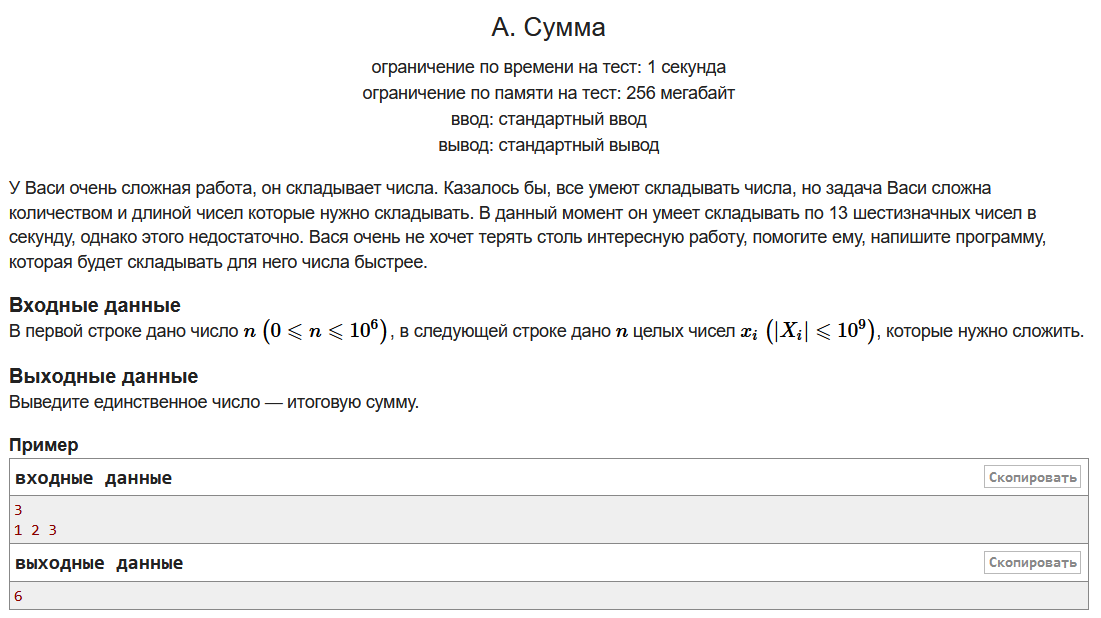
\includegraphics[width=\textwidth]{2A.png}
\end{center}
\subsubsection*{Идея решения}
Сначала заведем массив чисел и введем его через консоль с помощью цикла. Потом так же с помощью цикла просуммируем все числа в массиве и выведем ответ. Асимптотика $O(n)$, где $n$ - кол-во элементов. 
\subsubsection*{Исходный код}
\begin{lstlisting}
#include <iostream>
#include <string>
#include <unordered_map>
#include <unordered_set>
#include <algorithm>
#include <vector>
#include <cmath>
#include <iomanip>
using namespace std;
typedef long long ll;
int main()
{
	ios_base::sync_with_stdio(false);
	cin.tie(0);
	cout.tie(0);
	int n;
	cin >> n;
	ll ans = 0;
	for (int i = 0; i < n; i++) {
		ll x;
		cin >> x;
		ans += x;
	}
	cout << ans;
	return 0;
}
\end{lstlisting}
\subsubsection*{Фрагмент турнирной таблицы контеста}
\begin{center}
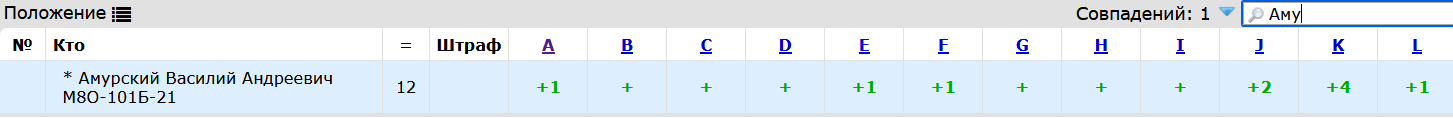
\includegraphics[width=\textwidth]{state2.png}\newline\noindent
\end{center}

\subsubsection*{Выводы}
Задача дорешана. Основные события отладки: неправильный ответ на претесте 1, забыл считать кол-во элементов в массиве.
\subsection*{Библиотека C++ [4]}
\begin{center}
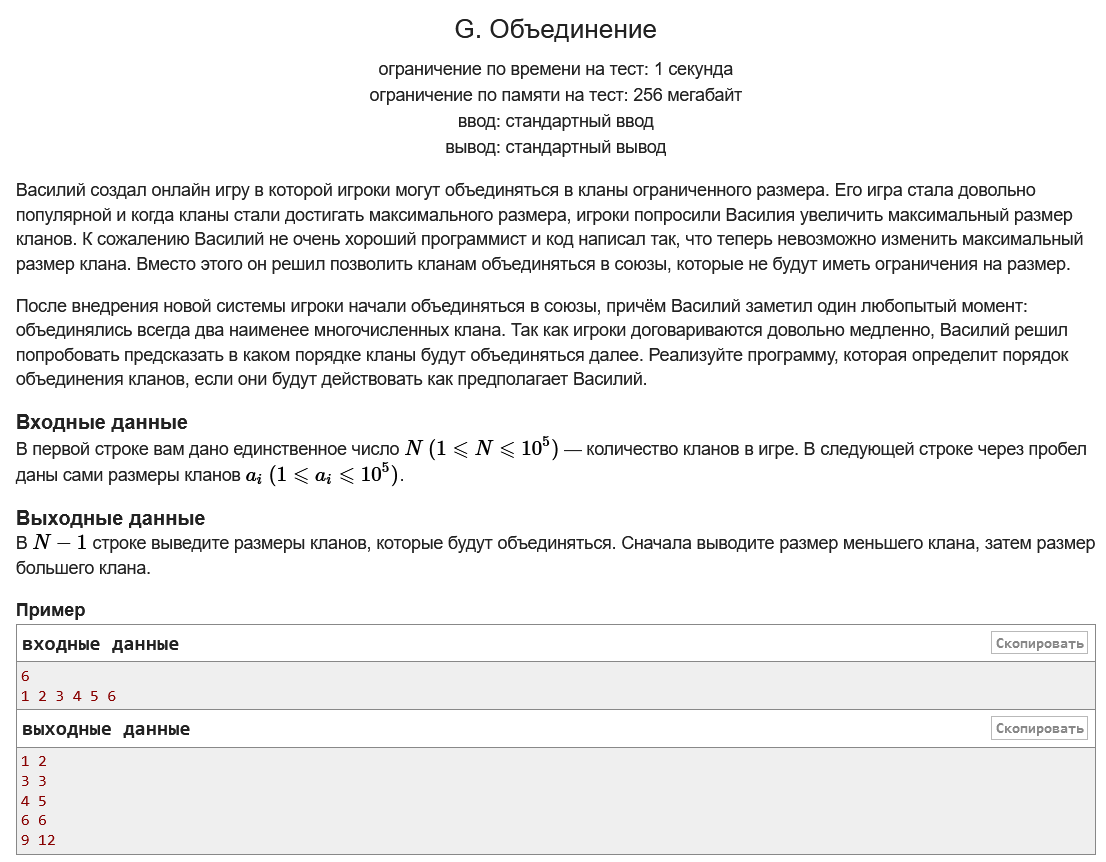
\includegraphics[width=\textwidth]{6G.png}
\end{center}
\subsubsection*{Идея решения}
Будем имитировать численность каждого клана в отсортированном состоянии благодаря типу multiset. Далее заведем цикл с $n-1$ итераций, где будем брать два минимальных элемента, выводить их и класть сумму в multiset. Асимптотика  $O(n\log{}n)$.
\subsubsection*{Исходный код}
\begin{lstlisting}
#include <iostream>
#include <string>
#include <unordered_map>
#include <unordered_set>
#include <map>
#include <set>
#include <algorithm>
#include <vector>
#include <cmath>
#include <iomanip>
using namespace std;
typedef long long ll;


int main()
{
    ios_base::sync_with_stdio(false);
    cin.tie(0);
    cout.tie(0);
    ll n;
    cin >> n;
    multiset<ll> a;
    for (int i = 0; i < n; i++) {
        ll x;
        cin >> x;
        a.insert(x);
    }
    for (int i = 0; i < n - 1; i++) {
        ll x1, x2;
        x1 = *a.begin();
        a.erase(a.begin());
        x2 = *a.begin();
        a.erase(a.begin());
        cout << x1 << ' ' << x2 << endl;
        a.insert(x1 + x2);
    }
    return 0;
}
\end{lstlisting}
\subsubsection*{Фрагмент турнирной таблицы контеста}
\begin{center}
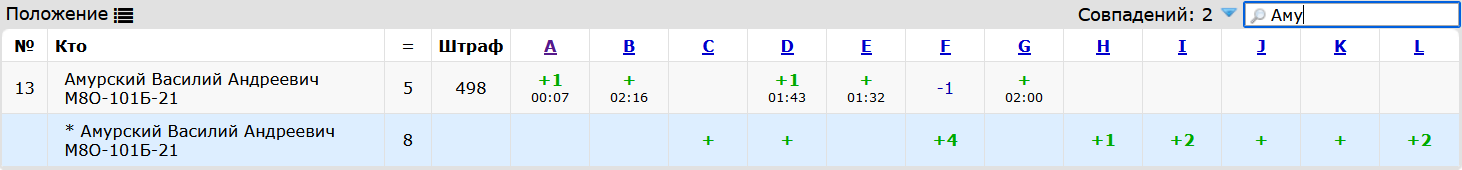
\includegraphics[width=\textwidth]{state6.png}\newline\noindent
\end{center}

\subsubsection*{Выводы}
Задача решена, проблем не возникло.
\subsection*{Арифметика в кольце, комбинаторика, функция Эйлера [7] }
\begin{center}
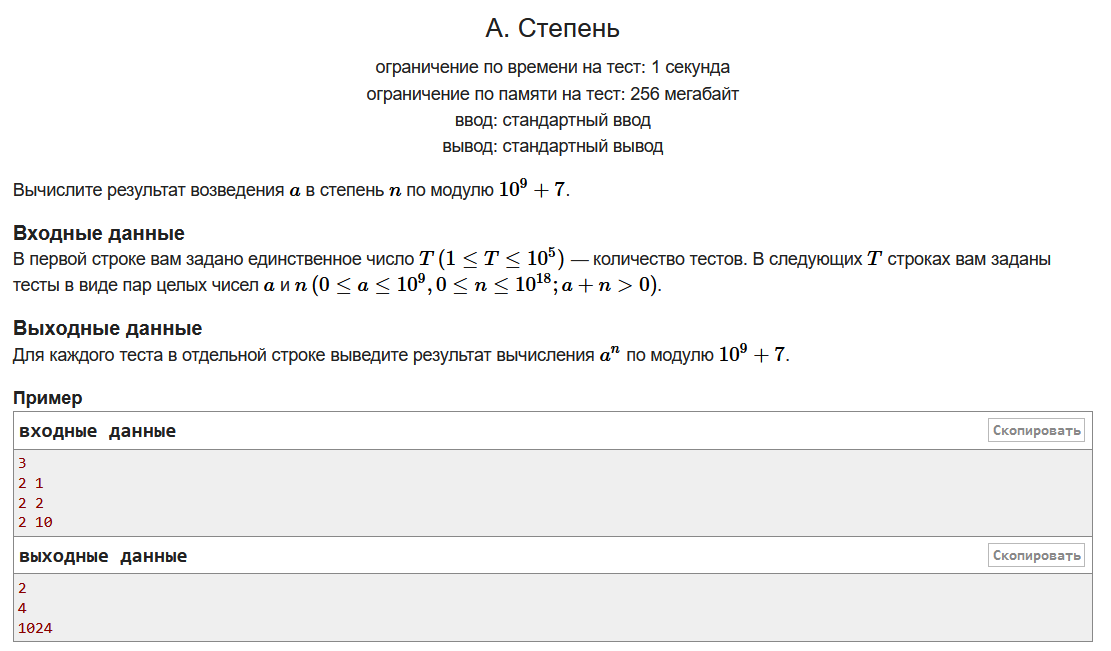
\includegraphics[width=\textwidth]{9A.png}
\end{center}
\subsubsection*{Идея решения}
Реализуем логарифмическое возведение в степень: от степени n мы переходим, если она чётна, к $n / 2$, а иначе — к $n-1$. Понятно, что всего будет не более $2 \log n$ переходов, прежде чем мы придём к $n = 0$. К тому же, после каждого перемножения будем брать остаток по $m=10^9+7$. Асимптотика $O(\log{}n)$
\subsubsection*{Исходный код}
\begin{lstlisting}
#include <iostream>
#include <string>
#include <unordered_map>
#include <unordered_set>
#include <map>
#include <set>
#include <algorithm>
#include <vector>
#include <cmath>
#include <numeric>
#include <iomanip>
#include <stack>
#include <fstream>
using namespace std;
typedef long long ll;
ll mod = 1000000007;
int main()
{
    ios_base::sync_with_stdio(false);
    cin.tie(0);
    cout.tie(0);
    ll t;
    cin >> t;
    for (int _ = 0; _ < t; _++) {
        ll res = 1;
        ll a, n;
        cin >> a >> n;
        while (n > 0) {
            if (n % 2 == 1) {
                res = (res * a) % mod;
            }
            a = (a * a) % mod;
            n /= 2;
        }
        cout << res << endl;
    }
    return 0;
}
\end{lstlisting}
\subsubsection*{Фрагмент турнирной таблицы контеста}
\begin{center}
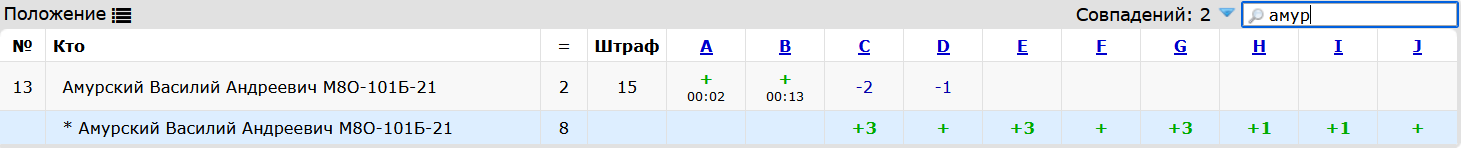
\includegraphics[width=\textwidth]{state9.png}\newline\noindent
\end{center}

\subsubsection*{Выводы}
Задача решена, проблем не возникло.
\subsection*{ Префиксные суммы, сортировка событий, метод двух указателей [8]}
\begin{center}
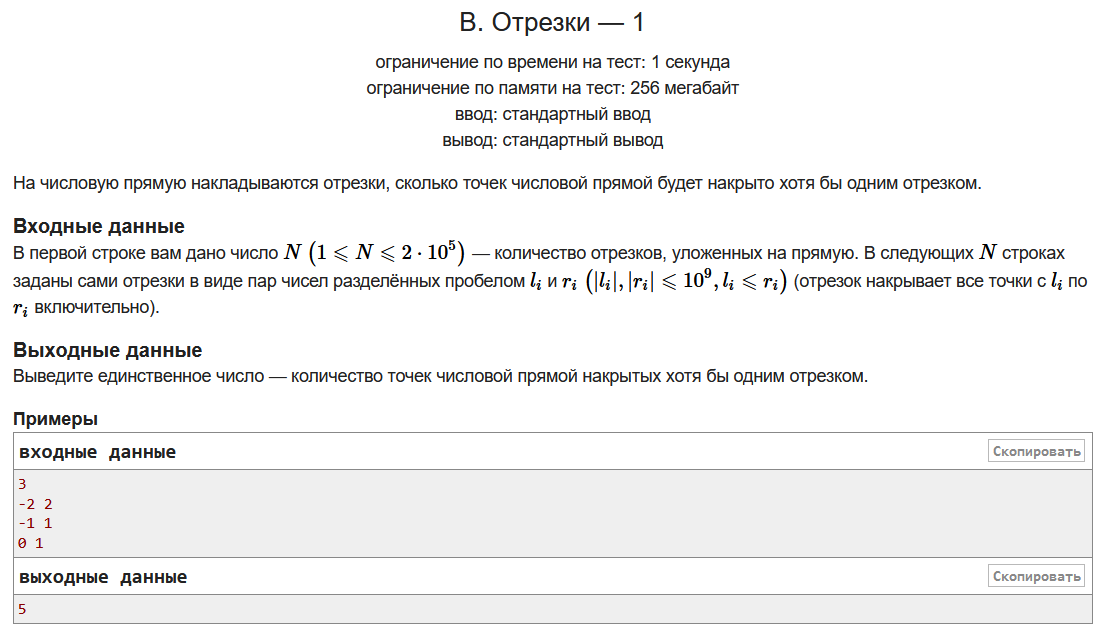
\includegraphics[width=\textwidth]{10B.png}
\end{center}
\subsubsection*{Идея решения}
Реализуем метод сканирующей прямой: создадим массив, в котором каждом элементе будет храниться два числа - первое число координата точки, второе число приоритет точки(0 - открывающая точка, 1 - закрывающая точка). К тому же будем хранить две переменные $ans$ и $q$, которые будут отвечать за кол-во точек не накрытых хотя бы одним отрезком и кол-во "открытых" отрезков. Далее будем обрабатывать сами отрезки: если текущая точка  открывающая, то добавим единицу к переменной $q$ и проверим равенство $q = 1$, если равенство справделиво, то добавим к переменной $ans$ разницу между текущей точкой и предыдущей, если точка закрывающая, то вычтем из $q$ единицу. Ответ равен $last - first - ans +1$, где $last$ - координата крайней правой точки, $first$ - координата крайней левой точки. Асимптотика $O(n\log{}n)$.
\subsubsection*{Исходный код}
\begin{lstlisting}
#include <iostream>
#include <cmath>
#include <algorithm>
#include <vector>
#include <iomanip>
#include <unordered_map>
#include <unordered_set>
#include <map>
#include <set>
#include <string>
#include <stack>
#include <deque>

using namespace std;
typedef long long ll;

int main() {
    ios_base::sync_with_stdio(false);
    cin.tie(0);
    cout.tie(0);
    ll n;
    cin >> n;
    vector<pair<ll, ll>> a(2*n);
    for (int i = 0; i < 2*n; i+=2) {
        ll l, r;
        cin >> l >> r;
        a[i] = { l, 0 };
        a[i + 1] = { r,1 };
    }
    sort(a.begin(), a.end());
    ll ans = 0;
    ll q = 0;
    for (int i = 0; i < 2 * n; i++) {
        if (a[i].second == 0) {
            ++q;
            if (q == 1 and i) {
                ans += a[i].first - a[i - 1].first - 1;
            }
        }
        else {
            --q;
        }
    }
    cout << a[2 * n - 1].first - a[0].first - ans + 1;
    return 0;
}
\end{lstlisting}
\subsubsection*{Фрагмент турнирной таблицы контеста}
\begin{center}
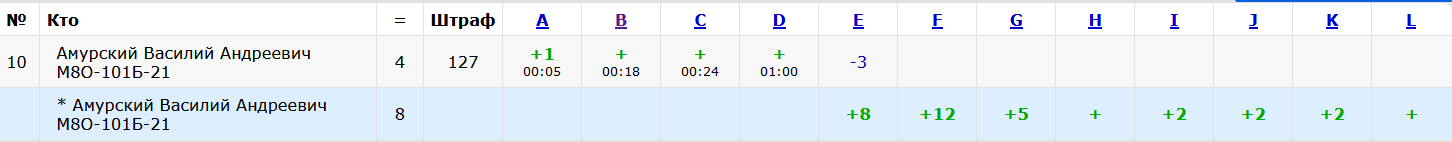
\includegraphics[width=\textwidth]{state10.png}\newline\noindent
\end{center}

\subsubsection*{Выводы}
Задача решена, проблем не возникло.
\subsection*{ Двумерное ДП, задача о рюкзаке [9]}
\begin{center}
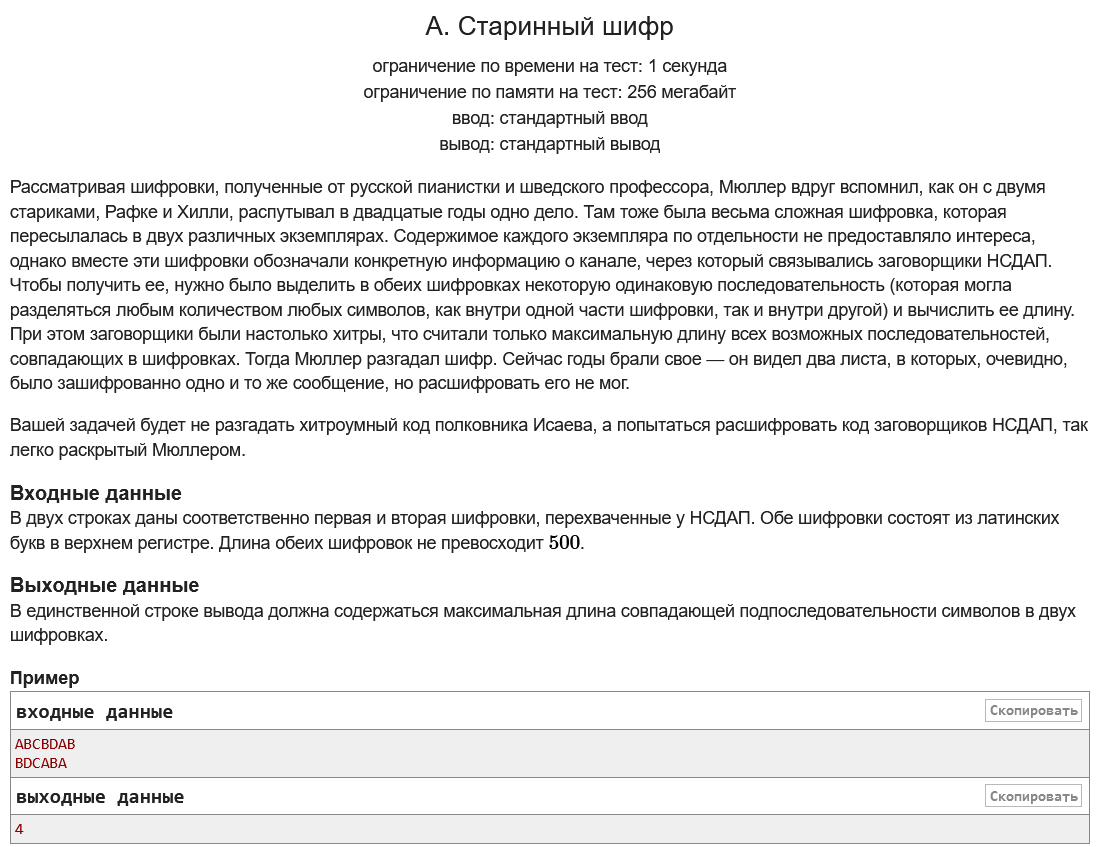
\includegraphics[width=\textwidth]{11A.png}
\end{center}
\subsubsection*{Идея решения}
Переборное решение будет работать за $O(n^2 * m^2)$, что при заданном условии не будет проходить ограничение по времени. При таком ограничении по времени зайдет только $O(n*m)$. Реализуем задачу о наибольшей общей возрастающей последовательности. $d[i][j]$ — это длина наибольшей общей возрастающей подпоследовательности префиксов $a[1..i]$ и $b[1..j]$, причем элемент $b[j]$ — последний представитель НОВП массива b, а $a[i]$ может не быть последним в массиве a. Вычислять d будем всё так же: сначала по увеличению i, а при равенстве — по увеличению j. Тогда для очередного значения $d[i][j]$ есть два варианта: 
\begin{itemize}
\item $a[i]$ не входит в НОВП. Тогда $d[i][j] = d[i-1][j]$: значение динамики уже посчитано на префиксе $a[1..i-1]$
\item $a[i]$ входит в НОВП. Это значит, что $a[i]=b[j]$, то есть для подсчёта $d[i][j]$ нужно пробегать циклом по b в поисках элемента $b[k]<b[j]$ с наибольшим значением $d[i-1][k]$. Но мы считаем d сначала по увеличению $i$, поэтому будем считать $a[i]$ фиксированным. Чтобы не запускать цикл при каждом равенстве $a[i]$ элементу $b[k]$, в дополнительной переменной best будем хранить "лучший" элемент (и его индекс ind в массиве b) такой, что этот элемент строго меньше $a[i]$ (а также меньше $b[k]$) и значение динамики для него максимально: $b[ind]<a[i]=b[j]$ и $best=d[i-1][ind] -> max$
\end{itemize}
\subsubsection*{Исходный код}
\begin{lstlisting}
#include <iostream>
#include <cmath>
#include <algorithm>
#include <vector>
#include <iomanip>
#include <unordered_map>
#include <unordered_set>
#include <map>
#include <set>
#include <string>
#include <stack>
#include <deque>

using namespace std;
typedef long long ll;

int main() {
    ios_base::sync_with_stdio(false);
    cin.tie(0);
    cout.tie(0);
    string a, b;
    cin >> a >> b;
    ll n = a.size(), m = b.size();
    vector<vector<ll>> dp(n + 1, vector<ll>(m + 1));
    for (int i = 1; i <= n; i++) {
        for (int j = 1; j <= m; j++) {
            if (a[i - 1] == b[j - 1]) {
                dp[i][j] = dp[i - 1][j - 1] + 1;
            }
            else {
                dp[i][j] = max(dp[i - 1][j], dp[i][j - 1]);
            }
        }
    }
    cout << dp[n][m];
    return 0;
}
\end{lstlisting}
\subsubsection*{Фрагмент турнирной таблицы контеста}
\begin{center}
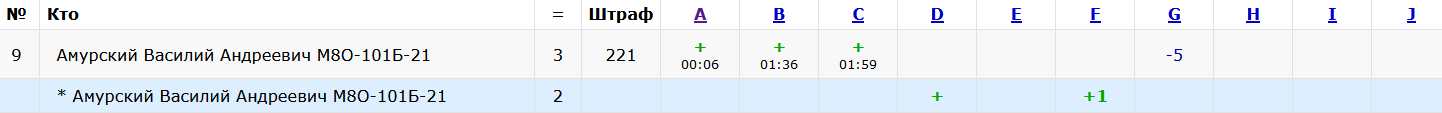
\includegraphics[width=\textwidth]{state11.png}\newline\noindent
\end{center}

\subsubsection*{Выводы}
Задача решена, проблем не возникло.
\subsection*{Геометрия, тернарный поиск [10]}
\begin{center}
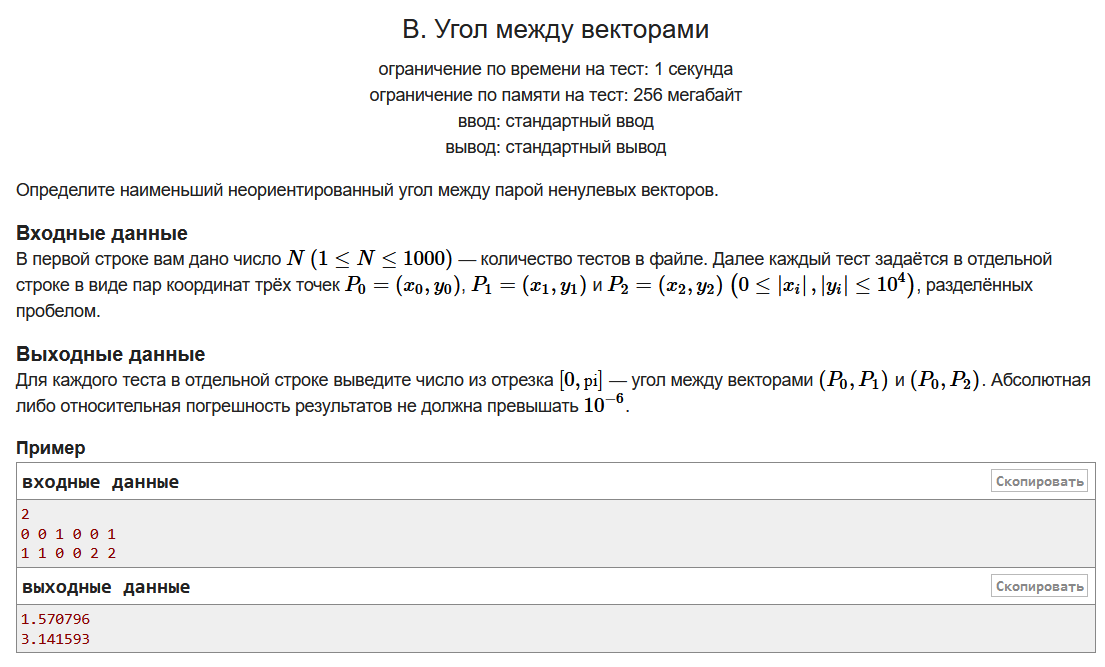
\includegraphics[width=\textwidth]{12B.png}
\end{center}
\subsubsection*{Идея решения}
Реализуем векторы и операции над ними. Угол между двумя векторами находится с помощью функции взятия арктангенса между векторным произведением и скалярным произведением, но здесь угол имеет диапазон от [$-2\pi; 2\pi$], а в условии сказано найти от $[0; \pi]$, поэтому возьмем модуль от полученного угла. Асимптотика $O(1)$.
\subsubsection*{Исходный код}
\begin{lstlisting}
#include <iostream>
#include <sstream>
#include <fstream>
#include <iomanip>
#include <string>
#include <cstdlib>
#include <cstdio>
#include <cstring>
#include <cmath>
#include <ctime>
#include <climits>
#include <cassert>
#include <vector>
#include <queue>
#include <stack>
#include <deque>
#include <set>
#include <map>
#include <bitset>
#include <utility>
#include <algorithm>
#include <unordered_map>
using namespace std;

const double eps = 10e-3;
struct point {
    double x, y;
    point() {}
    point(double a, double b) : x(a), y(b) {}
};

point operator -(const point& a, const point& b) {
    return point(a.x - b.x, a.y - b.y);
}

double scal(point a, point b) {
    return a.x * b.x + a.y * b.y;
}

double vec(point a, point b) {
    return a.x * b.y - b.x * a.y;
}

double ug(point a, point b) {
    return(atan2(vec(a, b), scal(a, b)));
}

double len(const point a, const point b) {
    return (sqrt((b.x - a.x) * (b.x - a.x) + (b.y - a.y) * (b.y - a.y)));
}

istream& operator >>(istream& in, point& p) {
    in >> p.x >> p.y;
    return in;
}

bool eql(double a, double b) {
    if (abs(a - b) < eps) {
        return true;
    }
    return false;
}

int main() {
    ios_base::sync_with_stdio(false);
    cin.tie(0);
    cout.tie(0);
    int n;
    cin >> n;
    for (int i = 0; i < n; i++) {
        point a, b;
        int x0, y0, x1, y1, x2, y2;
        cin >> x0 >> y0 >> x1 >> y1 >> x2 >> y2;
        a = point(x1 - x0, y1 - y0);
        b = point(x2 - x0, y2 - y0);
        cout << fixed << setprecision(6) << abs(ug(a, b)) << '\n';
    }
    return 0;
}
\end{lstlisting}
\subsubsection*{Фрагмент турнирной таблицы контеста}
\begin{center}
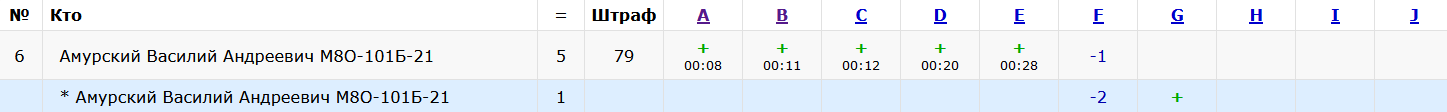
\includegraphics[width=\textwidth]{state12.png}\newline\noindent
\end{center}

\subsubsection*{Выводы}
Задача решена, проблем не возникло. 
\subsection*{Основы теории графов [11]}
\begin{center}
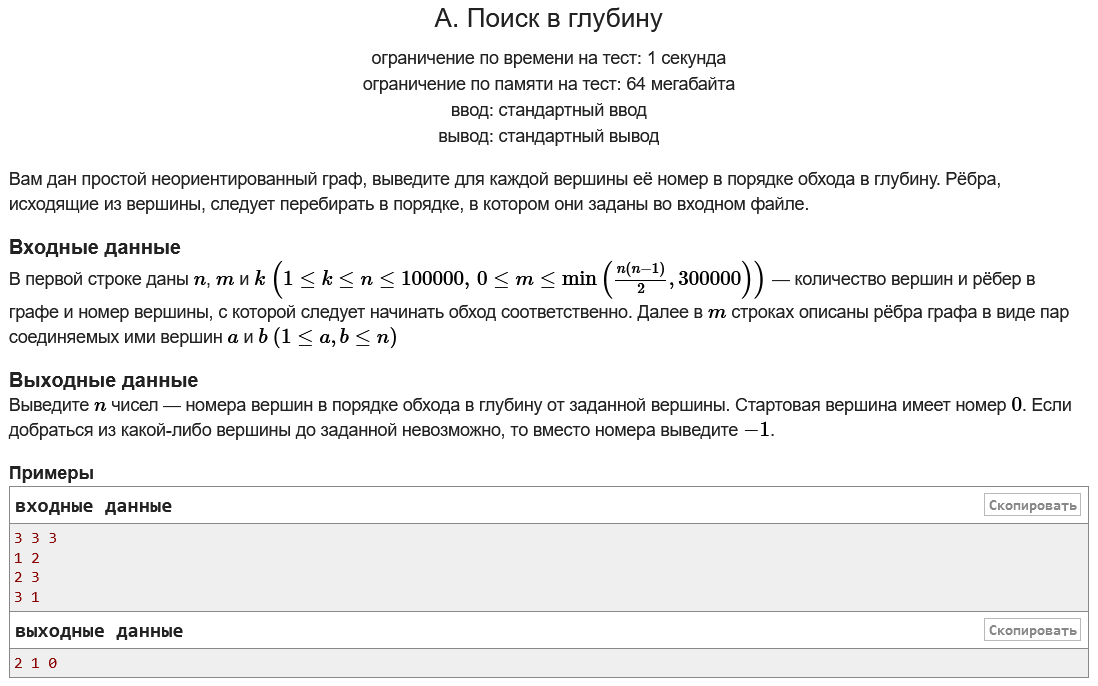
\includegraphics[width=\textwidth]{15A.png}
\end{center}
\subsubsection*{Идея решения}
Поиском в глубину называется рекурсивный алгоритм обхода дерева или графа, начинающий в корневой вершине (в случае графа её может быть выбрана произвольная вершина) и рекурсивно обходящий весь граф, посещая каждую вершину ровно один раз. Для того чтобы вывести вершины в порядке обхода в глубину заведем переменную счетчик $c$ и массив $ans$, где будем отмечать под каким значением счетчика мы вошли в вершину. В конце выведем массив $ans$.
\subsubsection*{Исходный код}
\begin{lstlisting}
#include <iostream>
#include <string>
#include <unordered_map>
#include <unordered_set>
#include <map>
#include <set>
#include <algorithm>
#include <vector>
#include <cmath>
#include <numeric>
#include <iomanip>
#include <stack>

using namespace std;
typedef   long long ll;

ll mod = 1000000007;
ll inf = INT64_MAX;

vector<vector<ll>> gr;
vector<bool> used;
vector<ll> ans;
ll c = 0;
void dfs( ll p) {
    used[p] = 1;
    ans[p] = c++;
    for (int i = 0; i < gr[p].size();i++) {
        if (!used[gr[p][i]]) {
            dfs(gr[p][i]);
        }
    }
}
int main() {
    ios_base::sync_with_stdio(false);
    cin.tie(0);
    cout.tie(0);
    ll n, m, k;
    cin >> n >> m >> k;
    gr.resize(n);
    used.resize(n);
    ans.assign(n, -1);
    for (int i = 0; i < m; i++) {
        ll a, b;
        cin >> a >> b;
        gr[a-1].push_back(b-1);
        gr[b - 1].push_back(a - 1);
    }
    dfs(k - 1);
    for (auto t : ans) {
        cout << t << ' ';
    }
    return 0;
}
\end{lstlisting}
\subsubsection*{Фрагмент турнирной таблицы контеста}
\begin{center}
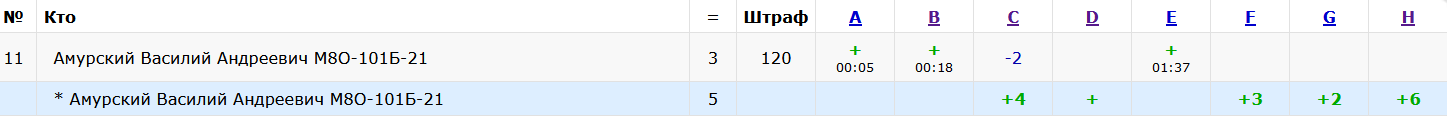
\includegraphics[width=\textwidth]{state15.png}\newline\noindent
\end{center}

\subsubsection*{Выводы}
Задача решена, проблем не возникло. 
\subsection*{Stage 10-B: Grand Prix of Kyoto, Div 2}
\begin{center}
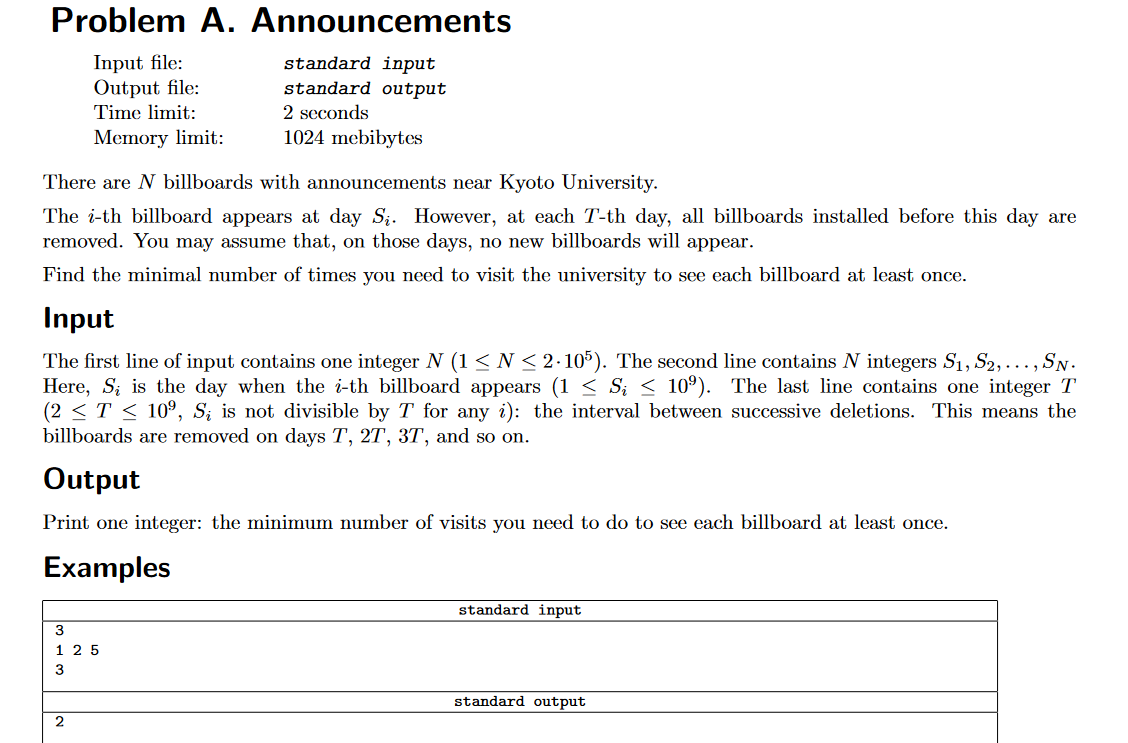
\includegraphics[width=\textwidth]{17A.png}
\end{center}
\subsubsection*{Идея решения}
Пусть одна итерация - это момент от предущего удаления листовок до следующего. Тогда мы можем узнать в какую итерацию была удалена каждая из листовок, поделив день вывешивания листовки на период их удаления. Нам надо узнать кол-во различных итераций. Это легко сделать, если мы результат деления положим в объект типа set и узнаем размер полученного множества. 
\subsubsection*{Исходный код}
\begin{lstlisting}
#include <iostream>
#include <cmath>
#include <vector>
#include <algorithm>
#include <set>
#include <queue>
#include <tuple>
#include <string>
#include <list>
typedef long long ll;
using namespace std;
const ll inf = INT64_MAX;

ll n, t;
vector<ll> a;

int main() {
	ios_base::sync_with_stdio(false);
	cin.tie(0);
	cout.tie(0);
	cin >> n;
	a.resize(n);
	for (int i = 0; i < n; i++) cin >> a[i];
	cin >> t;
	set<ll> ans;
	for (int i = 0; i < n; i++) {
		ans.insert(a[i] / t);
	}
	cout << ans.size();
	return 0;
}
\end{lstlisting}
\subsubsection*{Фрагмент турнирной таблицы контеста}
\begin{center}
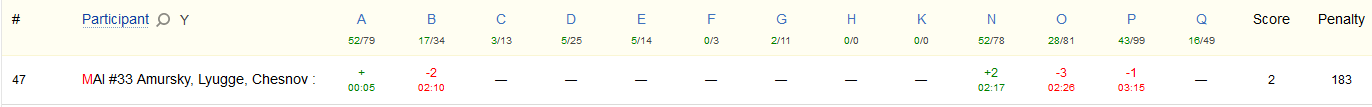
\includegraphics[width=\textwidth]{state17.png}\newline\noindent
\end{center}

\subsubsection*{Выводы}
Задача решена, проблем не возникло. 
\subsection*{Деревья, наименьший общий предок [14]}
\begin{center}
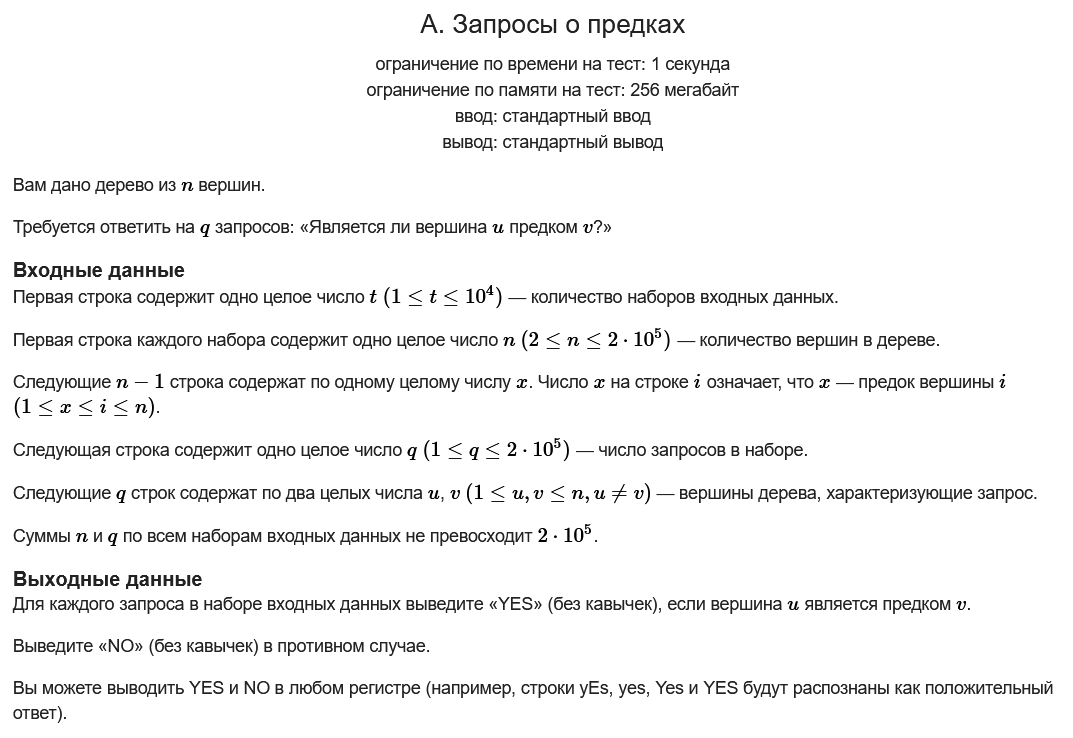
\includegraphics[width=\textwidth]{19A.png}
\end{center}
\subsubsection*{Идея решения}
Введем массивы $tin$ и $tout$ для подсчёта времени входа и выхода соотвественно. Вершина $u$ является предком $v$ тогда и только тогда, когда $tin_v \in [tin_u; tout_u]$. Это условие мы и проверим и выведем ответ. 
\subsubsection*{Исходный код}
\begin{lstlisting}
#include <iostream>
#include <sstream>
#include <fstream>
#include <iomanip>
#include <string>
#include <cstdlib>
#include <cstdio>
#include <cstring>
#include <cmath>
#include <vector>
#include <queue>
#include <algorithm>
using namespace std;
typedef int ll;
const long long size = 10e5 * 2 + 228;
ll n, m;
ll qq = 0;
ll q, v, u;
ll x;
int tin[202222], tout[202222];
vector<vector<ll>> gr;
void dfs(long long v, long long p = -1) {
    tin[v] = qq++;
    for (int i = 0; i < gr[v].size(); i++) {
        dfs(gr[v][i]);
    }
    tout[v] = qq;
    return;
}
int main() {
    ios_base::sync_with_stdio(false);
    cin.tie(0);
    cout.tie(0);
    ll t;
    cin >> t;
    for (int _ = 0; _ < t; _++) {
        cin >> n;
        gr.assign(n,vector<ll>());
       /* tin.assign(n,0), tout.assign(n,0);*/
        for (int i = 1; i <= n - 1; i++) {
            cin >> x;
            gr[x - 1].push_back(i);
        }
        dfs(0);
        cin >> q;
        for (int i = 0; i < q; i++) {
            cin >> u >> v;
            --u, --v;
            if (tin[v] >= tin[u] and tin[v] < tout[u]) {
                cout << "YES";
            }
            else cout << "NO";
            cout << '\n';
        }
      
    }
    return 0;
}
\end{lstlisting}
\subsubsection*{Фрагмент турнирной таблицы контеста}
\begin{center}
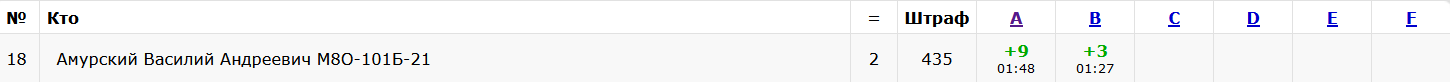
\includegraphics[width=\textwidth]{state19.png}\newline\noindent
\end{center}

\subsubsection*{Выводы}
Задача решена. Основные события процесса отладки: ошибка исполнения на тесте 2, вместо resize использовал assign; превышено ограничение времени на тесте 10, добавил команды cin.tie(0) и сout.tie(0);

\end{document}
